\documentclass{standalone}
\usepackage{tikz}
\usepackage{amsmath}
\usepackage{amssymb}

\begin{document}

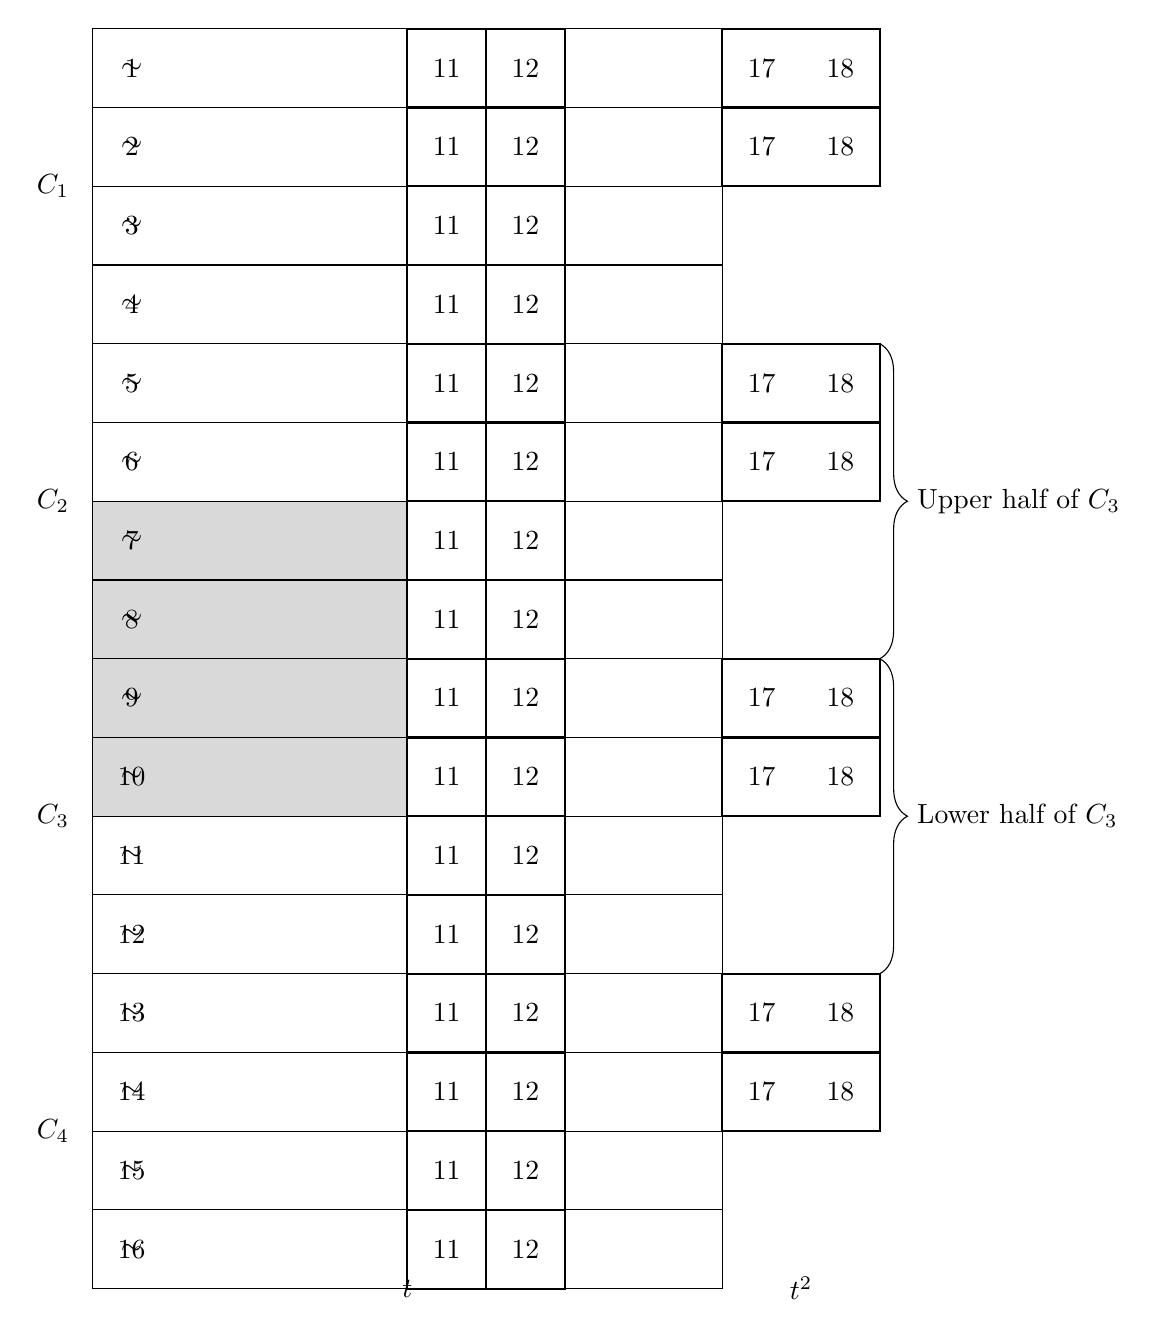
\begin{tikzpicture}
    % Define colors
    \filldraw[fill=gray!30] (0,-6) rectangle (4,-10);

    % C1 block
    \foreach \y in {0, -1, -2, -3} {
        \draw (0,\y) rectangle (8,\y-1);
        \node at (0.5,\y-0.5) {$\sim$};
    }
    \node at (0.5,-0.5) {$1$};
    \node at (0.5,-1.5) {$2$};
    \node at (0.5,-2.5) {$3$};
    \node at (0.5,-3.5) {$4$};

    % C2 block
    \foreach \y in {-4, -5, -6, -7} {
        \draw (0,\y) rectangle (8,\y-1);
        \node at (0.5,\y-0.5) {$\sim$};
    }
    \node at (0.5,-4.5) {$5$};
    \node at (0.5,-5.5) {$6$};
    \node at (0.5,-6.5) {$7$};
    \node at (0.5,-7.5) {$8$};

    % C3 block
    \foreach \y in {-8, -9, -10, -11} {
        \draw (0,\y) rectangle (8,\y-1);
        \node at (0.5,\y-0.5) {$\sim$};
    }
    \node at (0.5,-8.5) {$9$};
    \node at (0.5,-9.5) {$10$};
    \node at (0.5,-10.5) {$11$};
    \node at (0.5,-11.5) {$12$};

    % C4 block
    \foreach \y in {-12, -13, -14, -15} {
        \draw (0,\y) rectangle (8,\y-1);
        \node at (0.5,\y-0.5) {$\sim$};
    }
    \node at (0.5,-12.5) {$13$};
    \node at (0.5,-13.5) {$14$};
    \node at (0.5,-14.5) {$15$};
    \node at (0.5,-15.5) {$16$};

    % Highlight 11, 12
    \foreach \y in {0, -1, -2, -3, -4, -5, -6, -7, -8, -9, -10, -11, -12, -13, -14, -15} {
        \draw[thick] (4,\y) rectangle (5,\y-1);
        \draw[thick] (5,\y) rectangle (6,\y-1);
        \node at (4.5,\y-0.5) {11};
        \node at (5.5,\y-0.5) {12};
    }

    % Highlight 17, 18
    \foreach \y in {0, -1, -4, -5, -8, -9, -12, -13} {
        \draw[thick] (8,\y) rectangle (10,\y-1);
        \node at (8.5,\y-0.5) {17};
        \node at (9.5,\y-0.5) {18};
    }

    % Labels
    \node at (-0.5,-2) {$C_1$};
    \node at (-0.5,-6) {$C_2$};
    \node at (-0.5,-10) {$C_3$};
    \node at (-0.5,-14) {$C_4$};
    
    % Braces
    \draw[decorate,decoration={brace,amplitude=10pt}] (10,-4) -- (10,-8) node[midway,xshift=10pt,right] {Upper half of $C_3$};
    \draw[decorate,decoration={brace,amplitude=10pt}] (10,-8) -- (10,-12) node[midway,xshift=10pt,right] {Lower half of $C_3$};

    % Additional labels
    \node at (4,-16) {$t$};
    \node at (9,-16) {$t^2$};
\end{tikzpicture}

\end{document}